\chapter{Estado da arte}
\label{state}


Nesta capitulo, são apresentados os resultados da pesquisa bibliográfica sobre as ferramentas e funcionalidades que poderão estar presentes no sistema a desenvolver. Pretende-se apresentar de forma geral todas as tecnologias possíveis de utilização e respetiva comparação. 



\section{Conceitos tecnológicos}


Nesta secção são apresentados alguns conceitos tecnologias utilizados em toda a dissertação. Com o objetivo de não os repetir, estes serão descritos apenas aqui. 

\begin{itemize}
	\item \ac{HTML}: consiste numa linguagem de marcação que permite estruturar uma página web. 
	\item \ac{CSS}: permite personalizar os componentes existentes \ac{HTML}, isto é, personalizá-los com uma determinada cor, espaçamento ou fonte. 
	\item \ac{JS}: é uma linguagem de programação interpretada. Foi utilizada inicialmente para a criação de aplicações do lado do cliente, sendo que atualmente, já é bastante utilizada do lado do servidor. 
	
	\item Python: é uma  linguagem de programação de alto nível, possuindo os seguintes paradigmas:  orientação a objetos, programação imperativa, programação funcional. 
	
	
	\item \ac{API}: consiste numa interface de programação de aplicações, isto é, disponibiliza um conjunto de funções especificas que permitem ao programador aceder a determinadas funcionalidades.  
	
	\item Web Service: é um tipo de \ac{API} que trabalha com \ac{HTTP},
	ou \ac{SMTP}.
	
	
\end{itemize}



\section{\acl{SGBD}}

Um \acl{SGBD} (\acs{SGBD}) consiste num \textit{software} ou conjunto de \textit{softwares} responsáveis pela manipulação de uma base de dados, permitindo a realização de um conjunto enorme de operações, como por exemplo, operações básicas de manipulação de registos e respectiva visualização, operações estatísticas e respetivos relatórios, automatização de funcionalidades entre outros. Seguidamente são apresentados três \ac{SGBD} e a sua respetiva comparação. 


\subsection{MySQL}


O MySQL é considerado o \ac{SGBD} \textit{open source} mais popular de todo o mundo, sendo líder em aplicações baseadas na web, incluindo o Facebook, Twitter, YouTube, Yahoo! e muitos outros. Está comprovado que possui um elevado desempenho, fiabilidade e facilidade de utilização\cite{MySQL2011}.	






\subsection{SQL Server}

O SQL Server é um \ac{SGBD} desenvolvido pela Microsft com bastante popularidade, tendo suporto para as seguintes linguagens de programação C++, PHP, Java, \ac{JS}, Python entre outras. A ultima versão deste \ac{SGBD} é o SQL Server 2016, estando também disponível para ambiente Linux\cite{linuxsqlserver}.




\subsection{PostgreSQL}

O PostgreSQL é um sistema de gestão de base de dados do tipo objeto-relacional uma vez que permite um modelo de dados orientado a objetos, isto é, possibilita a manipulação de objetos, classes e heranças diretamente no esquemas da base de dados. Segundo o site oficial do PostgreSQL este é considerado um \ac{SGBD} bastante poderoso e com desenvolvimento \textit{open sources}\cite{ThePostgreSQLGlobalDevelopmentGroup2012}. 


%Ele tem mais de 15 anos de desenvolvimento ativo e uma arquitetura comprovada que ela ganhou uma forte reputação de confiabilidade, integridade de dados e correção. Ele roda em todos os principais sistemas operacionais, incluindo Linux, UNIX (AIX, BSD, HP-UX, SGI IRIX, MacOS, Solaris, Tru64), e Windows. É totalmente compatível com ACID, tem suporte completo para chaves estrangeiras, junções views, triggers e procedimentos armazenados (em várias línguas). Ele inclui mais SQL: 2008 tipos de dados, incluindo INTEGER, NUMERIC, BOOLEAN, CHAR, VARCHAR, DATE, INTERVALO e TIMESTAMP. Ele também suporta o armazenamento de grandes objetos binários, incluindo imagens, sons ou vídeo. Ele tem interfaces de programação nativas para C / C ++, Java, .Net, Perl, Python, Ruby, Tcl, ODBC, entre outros, e documentação



\subsection{Comparação e solução adotada}




A tabela \ref{Ranking-engines2016} encontra-se a classifica atribuída pela \textit{Ranking DB-Engines} para os \ac{SGBD} estudados de acordo com a sua popularidade, nos meses de Julho de 2017, Junho de 2017 e Julho de 2016\cite{DB-engines2016}. O MySQL é considerado o mais popular dos estudados, posteriormente o SQL Server e por fim o PostgreSQL. 

Uma vez que o cliente deste sistema pretende que sejam utilizadas tecnologias sem qualquer custo adicional, excluiu-se  desde logo o SQL Server da Microsoft. Restam então duas tecnologias estudadas: PostgreSQL e MySQL. Relatvivamente aos requisitos não funcionais do sistema, estes serão abordados mais à frente nesta dissertação. 



\newpage

\begin{table}[h]
	\centering

	\begin{tabular}{|
			>{\columncolor[HTML]{EFEFEF}}l |l|l|l|}
		\hline
		& \cellcolor[HTML]{EFEFEF}\textbf{Julho 2017} & \cellcolor[HTML]{EFEFEF}\textbf{Junho 2017} & \cellcolor[HTML]{EFEFEF}\textbf{Julho 2016} \\ \hline
		\textbf{MySQL} & 2º lugar & 2º lugar & 2º lugar \\ \hline
		\textbf{SQL Server} & 3º lugar & 3º lugar & 3º lugar \\ \hline
		\textbf{PostgreSQL} & 4º lugar & 4º lugar & 5º lugar \\ \hline
	\end{tabular}
	\caption[\textit{Ranking BD-Engines} para popularidade dos \ac{SGBD} estudados]{\textit{Ranking BD-Engines} para popularidade dos \ac{SGBD} estudados\cite{DB-engines2016}}
	\label{Ranking-engines2016}
\end{table}














Embora as diferenças entre estes os dois SGBD não sejam significativas, podemos também ter em consideração a performance. Para tal, foram realizados alguns estudos que pretendem comparar estas duas ferramentas usando a benchmark TPC-H\footnote{\url{http://www.tpc.org/tpch/}}, expondo que a performance do PostgreSQL é ligeiramente superior à do MySQL na maioria das queries\cite{Lopez2009}. %rever ref.  
A tabela \ref{comp-sqgbdcar} permite comparar algumas das características dos \ac{SGBD} estudados. 




\begin{table}[h]
	\centering

	\begin{tabular}{|
			>{\columncolor[HTML]{EFEFEF}}c |c|c|c|}
		\hline
		& \cellcolor[HTML]{EFEFEF}\textbf{MySQL} & \cellcolor[HTML]{EFEFEF}\textbf{SQL Server} & \cellcolor[HTML]{EFEFEF}\textbf{PostgreSQL} \\ \hline
		\textbf{Modelo} & \multicolumn{3}{c|}{Relacional} \\ \hline
		\textbf{Desenvolvido} & Oracle & Microsoft & \begin{tabular}[c]{@{}c@{}}PostgreSQL\\ Global Development Group\end{tabular} \\ \hline
		\textbf{Lançamento} & 1995 & 1989 & 1989 \\ \hline
		\textbf{Implementação} & C e C++ & C++ & C \\ \hline
		\textbf{Licença} & Open-source & Comercial & Open-source \\ \hline
		\textbf{Versão atual} & \begin{tabular}[c]{@{}c@{}}5.7.18\\ Abril 2017\end{tabular} & \begin{tabular}[c]{@{}c@{}}SQL Server 2016\\ Junho 2016\end{tabular} & \begin{tabular}[c]{@{}c@{}}9.6.3\\ Maio 2017\end{tabular} \\ \hline
		\textbf{Triggers} & \multicolumn{3}{c|}{Suporta} \\ \hline
		\textbf{\begin{tabular}[c]{@{}c@{}}Stored Procedures\\ e Functions\end{tabular}} & \multicolumn{3}{c|}{Suporta} \\ \hline
	\end{tabular}
	\caption{Comparação entre MySQL, SQL Server e PostgreSQL}
	\label{comp-sqgbdcar}
\end{table}



\section{Desenvolvimento web}



No que toca ao desenvolvimento web do sistema, permitindo que este seja adaptado ao cliente/empresa conforme as suas necessidades, poderão ser adotadas duas estratégias distintas: 

\begin{itemize}
	\item Por manipulação local utilizando \ac{JS} que interage com o \ac{DOM}. Exemplo de \textit{frameworks}: Angular.JS, Angular 2, React.JS, Vue.JS
	
	\item Por acesso ao servidor que servirá conteúdos criados em função dos pedidos do cliente. Exemplo de \textit{frameworks}: ASP.net, Django, Flask, Play, Spring
	
\end{itemize}


De modo a facilitar o desenvolvimento do sistema, optou-se que tanto  a nível de \textit{frontend} como de \textit{backend} este seja realizado paralelamente. Posto isto, será utilizada uma framework em que o servidor servirá os conteúdos em função das necessidade do cliente. Esta estratégia é mais eficiente e com tempos de resposta mais curtos, relativamente à primeira apresentada. De seguida, são apresentadas três \textit{frameworks} bastantes populares e com características distintas. 




\subsection{ASP.net}


ASP.net é uma tecnologia de \textit{scripting} que corre do lado do servidor, permitindo colocar numa página web, \textit{scripts} que irão ser executados por um determinado servidor. A sigla \acs{ASP} significa \acl{ASP}. Uma aplicação desenvolvida nesta tecnologia corre num servidor de Internet da Microsft, conhecido por \ac{IIS}, podendo ser desenvolvido recorrendo à linguagem C\# ou Microsoft Visual Basic. Esta tecnologia oferece três modelos para a criação de aplicações web, ASP.NET \textit{Web Forms}, ASP.NET \ac{MVC}, e ASP.NET \textit{Web Pages}, podendo ser criadas aplicações web estáveis e maduras com qualquer um deles\cite{Microsoft2016}. 


\subsection{Flask}


O Flask consiste numa micro-framework desenvolvida em Python baseado nas bibliotecas \ac{WSGI} Werkzeug e Jinja2\footnote{\url{http://jinja.pocoo.org/}}. Esta framework disponibiliza um  modelo simples para desenvolvimento web, um vez que permite economizar bastante tempo na sua conceção. De seguida, são apresentadas algumas das suas principais características\cite{Flask2014}. 


\begin{itemize}
	\item Possui um servidor para desenvolvimento e \textit{degub}
	\item Suporta testes unitários nativamente 
	\item Usa modelos da biblioteca Jinja2
	\item Suporta \textit{cookies} seguros (sessões do lado do cliente)
	\item Compatível com a primeira versão do \ac{WSGI}
	\item Baseado em unicode
	\item Extensa documentação 
\end{itemize}




\subsection{Django}


A framework Django consiste numa ferramenta de desenvolvimento web de alto nível desenvolvida na linguagem Python, possuindo uma arquitetura \ac{MVC}\cite{Deacon2005}, embora com algumas diferenças em relação a esta. No modelo \ac{MVC}, a componente \textit{Model} diz respeito à camada de acesso a dados, a \textit{View} à parte do sistema responsável pela escolha e apresentação da informação e o \textit{Controller} está encarregue de decidir que \textit{views} escolher. Os criadores do Django consideram a sua arquitetura com sendo \ac{MTV}\cite{Index}. 

\begin{itemize}
	\item \textit{Model}: é responsável por manipular, valiar, aceder e relacionar os dados. É considerada a fonte única e definitiva de informação (dados), possuindo os campos essenciais e os comportamentos sobre estes. Geralmente, cada \textit{Model} mapeia uma única tabela na base de dados. 
	
	
	\item \textit{Template}: é responsável pela apresentação dos dados. 

	\item \textit{View}: é responsável pela lógica de negócio e respetiva manipulação, acedendo ao Model e encaminhando o pretendido para o Template. 
	
\end{itemize}



De acordo com as descrições dos autores, esta ferramenta possui as seguintes vantagens\cite{Index}: 


\begin{itemize}
	\item Boa documentação;
	\item Facilidade e rapidez de desenvolvimento e \textit{deployment};
	\item Escalabilidade;
	\item Estabilidade.

\end{itemize}





\subsection{Conclusões e solução adotada}



Uma vez que o cliente do sistema não pretende que existam gasto adicionais, optou-se por utilizar ferramentas \textit{open-source} que permitiu desde logo excluir a tecnologia ASP.net. 


A escolha para desenvolvimento web recaiu sobre o Django uma vez que esta framework recomenda a utilização do PostgreSQL, indicando que permite alcançar um bom equilíbrio entre custo, características, rapidez e estabilidade\cite{Holovaty2009}. 













\newpage
\section{Desenvolvimento mobile}


http://bloomidea.com/blog/aplicacoes-nativas-vs-hibridas-qual-escolher-para-o-seu-projeto	

\subsection{Plataformas nativas}


uma aplicação móvel nativa é uma app que foi desenvolvida para ser utilizada numa plataforma ou dispositivo específico (iOS ou Android), usando as ferramentas e a linguagem de desenvolvimento correspondentes àquelas que o sistema em questão suporta. Uma app nativa pode assim interagir e tirar partido das funcionalidades do próprio sistema operativo e de outro software que esteja instalado nessa plataforma, o que faz desta opção uma excelente aposta.


\begin{itemize}
	\item \textbf{Performance}: 
	\item \textbf{Desenvolvimento}: 
	\item \textbf{Manutenção}: 
	\item \textbf{Interface}: 
	\item \textbf{Recursos disponíveis}: 
	\item \textbf{\textit{Plug-ins}}: 
	\item \textbf{Segurança}: 
\end{itemize}



\subsection{Multi-plataforma}

http://websocialdev.com/lista-de-frameworks-para-desenvolvimento-mobile/


\begin{itemize}
	\item \textbf{Performance}: 
	\item \textbf{Desenvolvimento}: 
	\item \textbf{Manutenção}: 
	\item \textbf{Interface}: 
	\item \textbf{Recursos disponíveis}: 
	\item \textbf{\textit{Plug-ins}}: 
	\item \textbf{Segurança}: 
\end{itemize}




\subsection{Conclusões e solução adotada}



Um vez que o cliente pretende uma solução mobile multiplataforma, isto é, possível de ser executada em IoS e Android optou-se por utilizar a framework Phonegap, sendo esta aconselhada pelo orientador Prof. Joaquim Sousa Pinto. 

Uma das principais desvantagens da utilização deste paradigma multiplataforma é o seu baixo desempenho na utilização de recursos do dispositivo. Uma que não será necessária essa utilização optou-se por utilizar a framework mencionada anteriormente. 



\newpage
\section{REST Frameworks}




\subsection{Django Rest Framework}





Django REST Framework é uma ferramenta considerada 'poderosa e flexível para a construção de APIs Web' [], que pode ser usada juntamente com a framework de desenvolvimento de aplicações Web Django, que quando integrada no desenvolvimento de um determinado \textit{backend} permite a implementação de serviços do tipo REST.



A API navegável Web é uma vitória usabilidade enorme para os desenvolvedores.

Políticas de autenticação , incluindo pacotes para OAuth1a e OAuth2 .

Serialização que suporta tanto ORM e não ORM fontes de dados.

Customizável todo o caminho - basta usar vistas regulares baseadas na função , se você não  precisar dos mais poderosos recursos .

Extensa documentação , e grande apoio da comunidade .

Utilizado e confiável por empresas internacionalmente reconhecidas, incluindo Mozilla , 
Red Hat , Heroku , e Eventbrite .




\subsection{Flask-RESTful}


\subsection{Restlet}



\subsection{Conclusões e solução adotada}




com autenticação via token 







app mobile
microcontroladores -> controller modulers 


documentação com swager 





\newpage
\section{Microcontroladores}


Um microcontrolador consiste numa solução integrada de um sistema computacional, num único dispositivo físico, sendo uma mistura de \textit{hardware} com \textit{software}. Possui vários módulos principais, um \ac{CPU} onde é realizado todo o processamento, as memórias de instrução e dados (\ac{RAM} e \ac{ROM}) e os portos de entrada e saída (\ac{I/O}), e ainda alguns periféricos (\textit{Timer}, \textit{Serial COM Port}). 

Estes dispositivos são responsáveis pelo processamento de dados, tomada de decisões, controlo do funcionamento de alguns módulos, mostra e conversão da informação recolhida pelos sensores, entre outros. Com o objetivo de simular o sistema que será apresentado, serão utilizados dois microcontroladores bastante comuns no mercado, um Arduino Nano e um Raspberry Pi 3.  


\subsection{Arduino Nano}


Como descrito no site oficial, um Arduino consiste numa plataforma \textit{open-source} de prototipagem eletrónica composta por \textit{hardware} e \textit{software} flexíveis e com elevada facilidade utilização. Esta plataforma é utilizada para projetos especialmente no contexto do \ac{IoT} e da robótica educativa, sendo possível de incorporar vários módulos, dependendo da tarefa que se quer que seja executada\cite{Banzi2012}. 

Na figura \ref{ard2} e \ref{ard1} apresenta-se uma imagem do Arduino utilizado e a identificação dos diferentes pinos existentes, respectivamente. 


\begin{figure}[h]
	\centering
	\begin{minipage}[b]{0.49\textwidth}
		\centering
		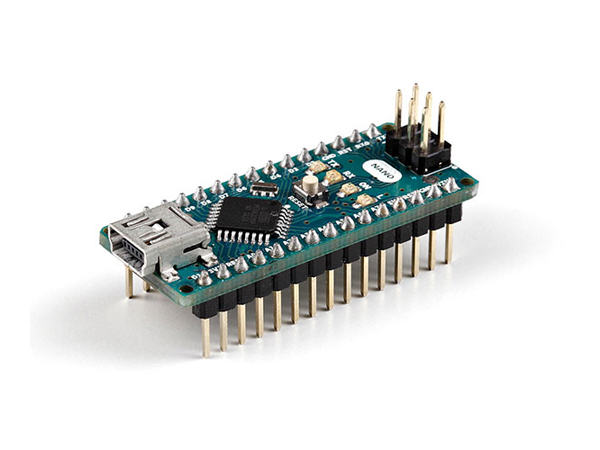
\includegraphics[width=\textwidth]{img/hardware/nano-img.jpg}
		\caption{Arduino Nano}
		\label{ard2}
	\end{minipage}
	\hfill
	\begin{minipage}[b]{0.49\textwidth}
		\centering
		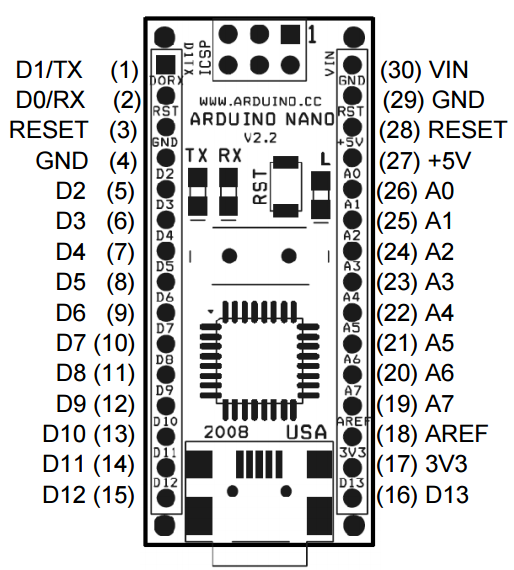
\includegraphics[width=0.6\textwidth]{img/hardware/nano-esquema.png}
		\caption[Identificação dos pinos num Arduino Nano]{Identificação dos pinos num Arduino Nano (Retirado de \cite{arduinonanouser})}
		\label{ard1}
	\end{minipage}
\end{figure}



O Arduino Nano possui um conjunto de pinos que podem ser programados para funcionarem como entradas ou saídas fazendo com que este  microcontrolador interaja com o meio externo para os mais diversos fins. Para além dos pinos de \ac{I/O} exitem pinos de alimentação que fornecem diversos valores de tensão que podem ser utilizados para transmitir energia elétrica aos diferentes componentes de um projeto\cite{Banzi2012}. Na tabela \ref{caraarduino} encontram-se as principais características desta versão do Arduino. 




\begin{table}[h]
	\centering
	
	\begin{tabular}{|
			>{\columncolor[HTML]{EFEFEF}}l |l|} \hline
		\textbf{Microcontrolador} & ATmega328 \\ \hline
		\textbf{Tensão de operação} & 5V \\ \hline
		\textbf{Tensão de entrada} & 7-12V \\ \hline
		\textbf{Portas digitais} & 14 (6 podem ser usadas como PWM) \\ \hline
		\textbf{Portas analógicas} & 8 \\ \hline
		\textbf{Corrente nos pinos} \ac{I/O} & 40mA \\ \hline
		\textbf{Memória Flash} & 32KB (2KB usado no bootloader) \\ \hline
		\textbf{Memória \acs{RAM} (SRAM)} & 2KB \\ \hline
		\textbf{EEPROM} & 1KB \\ \hline
		\textbf{Velocidade do \textit{Clock}} & 16MHz \\ \hline
		\textbf{Dimensões} & 45 x 18mm \\ \hline
		\textbf{\ac{LED} interno} & Pino digital 13 \\ \hline
		\textbf{Ligação \ac{USB}} & Ligação ao computador e alimentação \\ \hline
	\end{tabular}
	\caption[Características do Arduino Nano]{Características do Arduino Nano (Adaptado de \cite{Melorose2015})}
	\label{caraarduino}
\end{table}






\subsection{Raspberry Pi 3}

Um Raspberry Pi (figura \ref{rasp1}) comparativamente com outros dispositivos de igual dimensão é mais poderoso e já incorpora alguns periférico \ac{I/O}, tal como um computador normal. Tem o tamanho de um cartão de crédito que possui um conjunto de \textit{hardware} integrado que tal como Arduino possibilita uma interação com o meio exterior. Este dispositivo pode ser ligado a um monitor através da saída HDMI, possuindo ainda uma saída de áudio e várias portas \ac{USB}, tendo sido desenvolvido no Reino Unido pela \textit{Raspberry Pi Foundation}. Este microcontrolador é compatível com sistemas operativos baseados em GNU/Linux, sendo que no trabalho prático desta dissertação se encontra instalada a versão Raspbian\footnote{Distribuição Linux oficial do Raspberry Pi:  \url{https://www.raspberrypi.org/downloads/raspbian/}}\cite{RaspberryPiFoundation2012}. 




\begin{figure}[h]
	\centering
	\begin{minipage}[b]{0.49\textwidth}
		\centering
		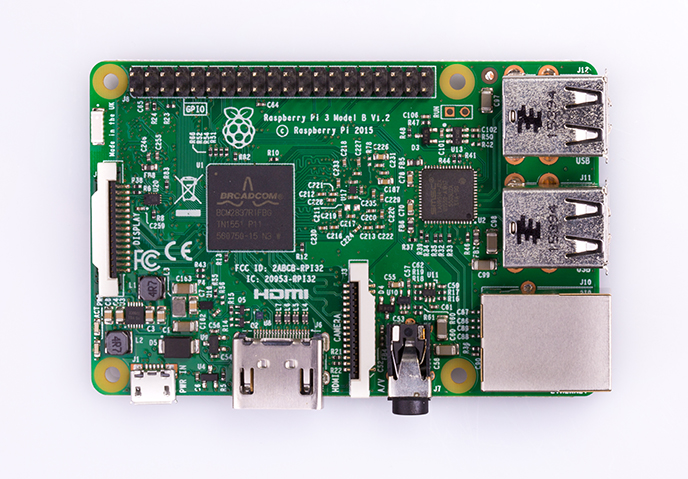
\includegraphics[width=\textwidth]{img/hardware/rasp3-img.jpg}
		\caption{Raspberry Pi 3}
		\label{rasp1}
	\end{minipage}
	\hfill
	\begin{minipage}[b]{0.49\textwidth}
		\centering
		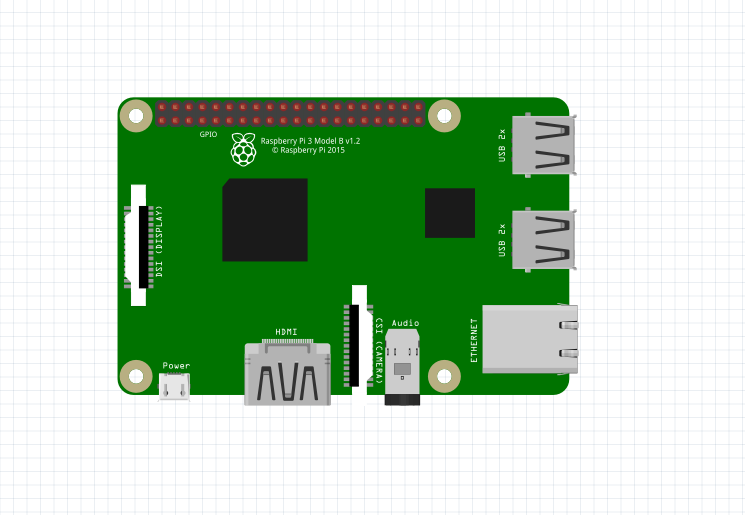
\includegraphics[width=0.8\textwidth]{img/hardware/rasp-esquema.PNG}
		\caption{Principais componentes no Raspberry Pi 3 }
		\label{comprasp1}
		
	\end{minipage}
\end{figure}


No trabalho prático desta dissertação será utilizada a versão 3 do Raspberry Pi, tendo este surgido em fevereiro de 2016. Na figura \ref{comprasp1} encontram-se os principais componentes desta versão. Seguidamente, na tabela \ref{comp23} é feita um comparação entre a versão 2 e 3 do Raspberry Pi. 




\begin{table}[h]
	\centering
	\begin{tabular}{|
			>{\columncolor[HTML]{EFEFEF}}l |l|l|}
		\hline
		& \cellcolor[HTML]{EFEFEF}\textbf{Raspberry Pi 2 Model B 1.2} & \cellcolor[HTML]{EFEFEF}\textbf{Raspberry Pi 3 Model B} \\ \hline
		\textbf{CPU} & QUAD Core 900MHz & QUAD Core 1.2GHz \\ \hline
		\textbf{RAM} & 1GB SDRAM & 1GB SDRAM \\ \hline
		\textbf{Potência máxima} & 5V/1.8A & 5V/2.5A \\ \hline
		\textbf{Armazenamento} & MicroSD & MicroSD \\ \hline
		\textbf{USB 2.0} & 4 x Portas USB & 4 x Portas USB \\ \hline
		\textbf{GPIO} & 40 pinos & 40 pinos \\ \hline
		\textbf{Porta Ethernet} & Sim & Sim \\ \hline
		\textbf{Wifi} & Incorporado (versão 802.11n) & Não \\ \hline
		\textbf{Bluetooth LE} & Incorporado (versão 4.1) & Não \\ \hline
	\end{tabular}
	\caption{Comparação entre versão 2 e 3 do Raspberry Pi}
	\label{comp23}
\end{table}









\section{Sensores}


Esta secção tem como objetivo fazer um estudo comparativo entre as diferentes tecnologias usadas para a medição dos vários parâmetros ambientais necessários ao controlo e monitorização da Salicórnia. Serão descritos alguns sensores de temperatura, luminosidade e salinidade. 



\subsection{Sensor de temperatura }
Existem vários tipos de sensores de temperatura baseados em princípios de funcionamento distintos.  

\begin{itemize}
	\item \textbf{Termopares}: são sensores de temperatura simples, robustos e de baixo custo, constituídos por duas partes diferentes de material condutor. Podem medir temperaturas entre os -200ºC e os 2315ºC, sendo usados em grande escala no meio industrial\cite{REOTEMPInstrumentCorporation}. 
	 
	
	\item \textbf{Termístor}: são sensores cuja resistência varia com a temperatura, sendo construídos a partir de materiais semicondutores. Um termístor detêm uma maior sensibilidade, pois a sua característica exponencial possibilita que uma pequena variação de temperatura traga uma grande variação na sua resistência, permitindo que a temperatura típica seja entre os -100ºC e os 300ºC. Estes sensores são frágeis, baratos e de reduzidas dimensões, sendo suscetíveis a problemas de auto aquecimento\cite{TemperatureSensors}.
	

	\item \textbf{Circuito integrado}: são sensores construidos através de materiais semicondutores, o que possibilita que tenham uma gama de temperatura limitada, geralmente entre os -55ºC e os 150ºC. 	Estão disponíveis com saídas em tensão, ou corrente, linearmente proporcional à temperatura. 


\end{itemize}





\subsection{Sensor de luminosidade }


%O LDR (Light Dependent Resistor) é um componente cuja resistência varia de acordo com a intensidade da luz. Quanto mais luz incidir sobre o componente, menor a resistência. Este sensor de luminosidade pode ser utilizado em projetos com arduino e outros microcontroladores para alarmes, automação residencial, sensores de presença e etc.


Existe uma variedade enorme de sensores de luminosidade/radição no mercado, contudo para monitorizar a luminosidade incidente numa planta é fundamental conhecer a radiação que é utilizada no processo de fotossíntese, denominada por \ac{PAR}. A figura \ref{grapFoto} ilustra que as plantas são mais sensíveis à luz azul e vermelha, estando essa radiação compreendida entre os  300nm e os 700nm. De seguida são apresentados alguns dos tipos de sensores mais comuns no mercado. 





\begin{figure}[!htb]
	\centering
	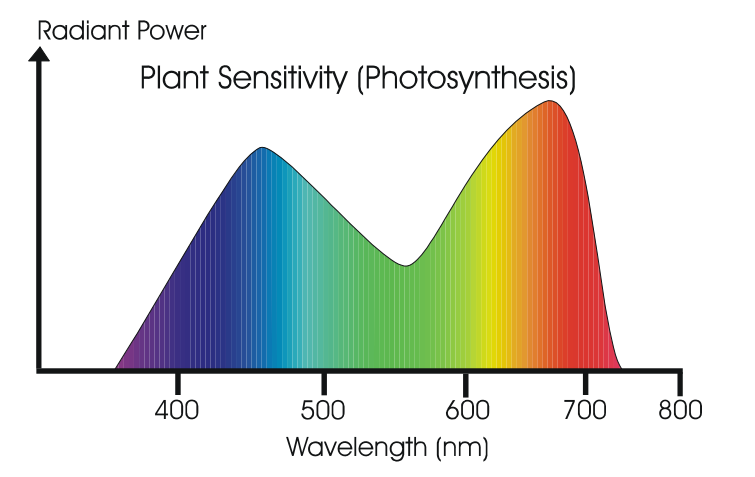
\includegraphics[scale=0.3]{img/plantagrap.png}
	\caption[Sensibilidade luminosa nas plantas durante a fotossíntese)]{Sensibilidade luminosa nas plantas durante a fotossíntese (Retirado de \cite{Argus2010})}
	\label{grapFoto}
\end{figure}




\begin{itemize}
	\item \textbf{Sensores \ac{PAR}}: são desenhados especificamente para medir radiação fotosintética ativa, sendo indicados para medir a luz incidente numa planta. São sensores muito caros sendo utilizados maioritariamente na investigação hortícola. 
	


	
	
	
	\item \textbf{Piranómetros}: estes sensores mede a radiação solar total (radiação ultravioleta, visível e infravermelha), devendo ser utilizados no exterior, sendo particularmente úteis em estações meteorológicas. Estes tipo de sensores são bastante dispendiosos, podendo ser mais caros dos que os sensores \ac{PAR}. 
	
	
	
	
	\item \textbf{Sensores optoelectrónicos}: são dispositivos eletrónicos que se baseiam em fenómenos fotovoltaicos. Seguidamente são destacados três sensores deste tipo, possuindo um elevado desempenho quando afetado por ruído e uma elevada sensibilidade. São considerados os sensores de luminosidade mais económicos.  
	 
		\begin{itemize}
			\item \textbf{Fotodíodo}: pode ser visto como um díodo comum, gerando uma corrente ou tensão quando incide radiação sobre ele.
			\item \textbf{Fototransístor}: é um transístor desenhado para receber luz, normalmente num módulo transparente.
			\item \textbf{\ac{LDR}}: trata-se de um material semicondutor cuja resistência diminui com a incidência de luz. 
		\end{itemize}
	
\end{itemize}





\subsection{Sensor de salinidade}


Atualmente ainda não há disponível nenhum sensor que permite medir exatamente a salinidade, mas existem sensores que medem a condutividade elétrica num determinado meio, permitindo concluir o estado do meio relativamente à quantidade de sal existente. 
Um exemplo disso, é o sensor SAL-BTA da Vernier\cite{sall} que permite medir de forma fácil e precisa o teor de sal dissolvido numa solução aquosa.




\section{Tecnologias de comunicação}

Nesta secção serão apresentados alguns das tecnologias de comunicação mais utilizados em \textit{Internet of Things} que permite a troca de informações entre dispositivos. Serão abordados quatro tecnologias de comunicação:  







\subsection{Zigbee}

Zigbee designa um conjunto de especificações para a comunicação sem-fio entre dispositivos eletrônicos, com ênfase na baixa potência de operação, na baixa taxa de transmissão de dados e no baixo custo de implementação. Tal conjunto de especificações define camadas do modelo OSI subsequentes àquelas estabelecidas pelo padrão IEEE 802.15.4.









\subsection{Bluetooth (BLE)}

Bluetooth é uma especificação de rede sem fio de âmbito pessoal (Wireless personal area networks – PANs) consideradas do tipo PAN ou mesmo WPAN


\subsection{Wi-Fi (IEEE 802.11)}

rede sem fio IEEE 802.11, que também são conhecidas como redes Wi-Fi ou wireless, foram uma das grandes novidades tecnológicas dos últimos anos. Atuando na camada física, o 802.11 define uma série de padrões de transmissão e codificação para comunicações sem fio, sendo os mais comuns: FHSS (Frequency Hopping Spread Spectrun), DSSS (Direct Sequence Spread Spectrum) e OFDM (Orthogonal Frequency Division Multiplexing). Atualmente, é o padrão de fato em conectividade sem fio para redes locais. Como prova desse sucesso pode-se citar o crescente número de Hot Spots e o fato de a maioria dos computadores portáteis novos já saírem de fábrica equipados com interfaces IEEE 802.25. A Rede IEEE possui como principal característica transmitir sinal sem fio através de ondas!









Baseado no standard IEEE 802.11, o Wi-Fi é uma tecnologia de transmissão e receção de dados sem fios. Ao longo dos anos têm surgido diferentes variantes do mesmo standard, sendo
a variante 802.11g a mais comum e aqui apresentada.
Aprovada a Junho de 2003 , a variante Wi-Fi tem as seguintes características principais
[82, 83]:

\begin{itemize}
	\item Banda de frequência de 2.4 GHz;
	\item Taxa de bits máxima de 54 Mbps na camada física, transferência de dados máxima de 24.7 Mbps;
	\item Topologia ponto-a-ponto (ad-hoc) e estrela (infraestrutura) suportadas;
	\item Vários mecanismos de encriptação e autenticação;
\end{itemize}




[82] IEEE 802.11g Wi-Fi Tutorial, Ian Poole, Radio Electronics. Visitado a Outubro de 2015.
URL: http://www.radio-electronics.com/info/wireless/wi-fi/ieee-802-11g.php
[83] The New Mainstream Wireless LAN Standard, Broadcom. Visitado a Outubro de 2015.
%URL: http://www.dell.com/downloads/global/shared/broadcom_802_11_g.pdf


\subsection{Sigfox}

Uma empresa francesa que constrói redes sem fio para conectar objetos de baixa energia, como medidores de energia elétrica , smartwatches e máquinas de lavar, que precisam estar continuamente ligados e emitindo pequenas quantidades de dados. Sua tecnologia é voltada para a Internet das Coisas (IoT).


\subsection{Comparação de tecnologias de comunicação}




\begin{table}[h]
	\centering

	\begin{tabular}{|
			>{\columncolor[HTML]{EFEFEF}}l |l|l|l|l|}
		\hline
		& \cellcolor[HTML]{EFEFEF}\textbf{Zigbee} & \cellcolor[HTML]{EFEFEF}\textbf{Bluetooth} & \cellcolor[HTML]{EFEFEF}\textbf{Wi-fi} & \cellcolor[HTML]{EFEFEF}\textbf{Sigfox} \\ \hline
		\textbf{IEEE} & 802.15.4 & 802.15.1 & 802.11n & N/A \\ \hline
		\textbf{Banda de frequência} & \begin{tabular}[c]{@{}l@{}}868/915 MHz\\ 2.4 GHz\end{tabular} & 2,4-5,5 GHz & 2,4-5 GHz & \begin{tabular}[c]{@{}l@{}}800 Hz\\ (europa)\end{tabular} \\ \hline
		\textbf{Topologia da rede} & Mesh & Estrela & Estrela & P2P \\ \hline
		\textbf{Energia (consumo)} & Muito baixo & Baixo & Médio & Muito baixo \\ \hline
		\textbf{Alcance} & 10m & aprox. 50m & 100m & \begin{tabular}[c]{@{}l@{}}Rural: 10-15m\\ Urbano: 3-5m\end{tabular} \\ \hline
		\textbf{Bateria (duração)} & Meses-anos & Dias & Horas & 10/15 anos \\ \hline
		
	\end{tabular}
	\caption{Comparação entre tecnologias de comunicação}
	\label{com-tecn}
\end{table}




Artigo: \cite{Rahman2015}



%\subsection{Módulo bluetooth}







\newpage
\section{Aplicações relacionadas}



Seja para comparar, seja para replicar boas funcionalidades, ou seja para conseguir oferecer algo mais ao utilizador final, quando se pretende desenvolver uma determinada aplicação, e
importante proceder a uma avaliação de aplicações da mesma área se encontram no mercado.
Assim, são aqui abordadas algumas das aplicações relacionadas que são mais utilizadas ou que mais se aproximam daquilo que se pretende para a aplicação a desenvolver neste projeto,
tendo em conta os diferentes sistemas operativos.



\subsection{Multi-monitorização de estufas agrícolas }

https://repositorio.ipcb.pt/bitstream/10400.11/949/1/Multimonitorizacao%20Estufa%20Agricola.PDF

\subsection{Agroopar}

http://www.vidarural.pt/agroopar-os-custos-na-mao-do-agricultor/


\subsection{outras que vale a pena para comparacao..}

%\subsection{Sistema de Monitorização de Estufas Agrícolas}


http://www.anje.pt/preview/perfil-coolfarm



\cite{Abreu2012}


\newpage









